\subsection{Цианидные комплексы 8 и 10 групп}

\begin{figure}[H]
\centering
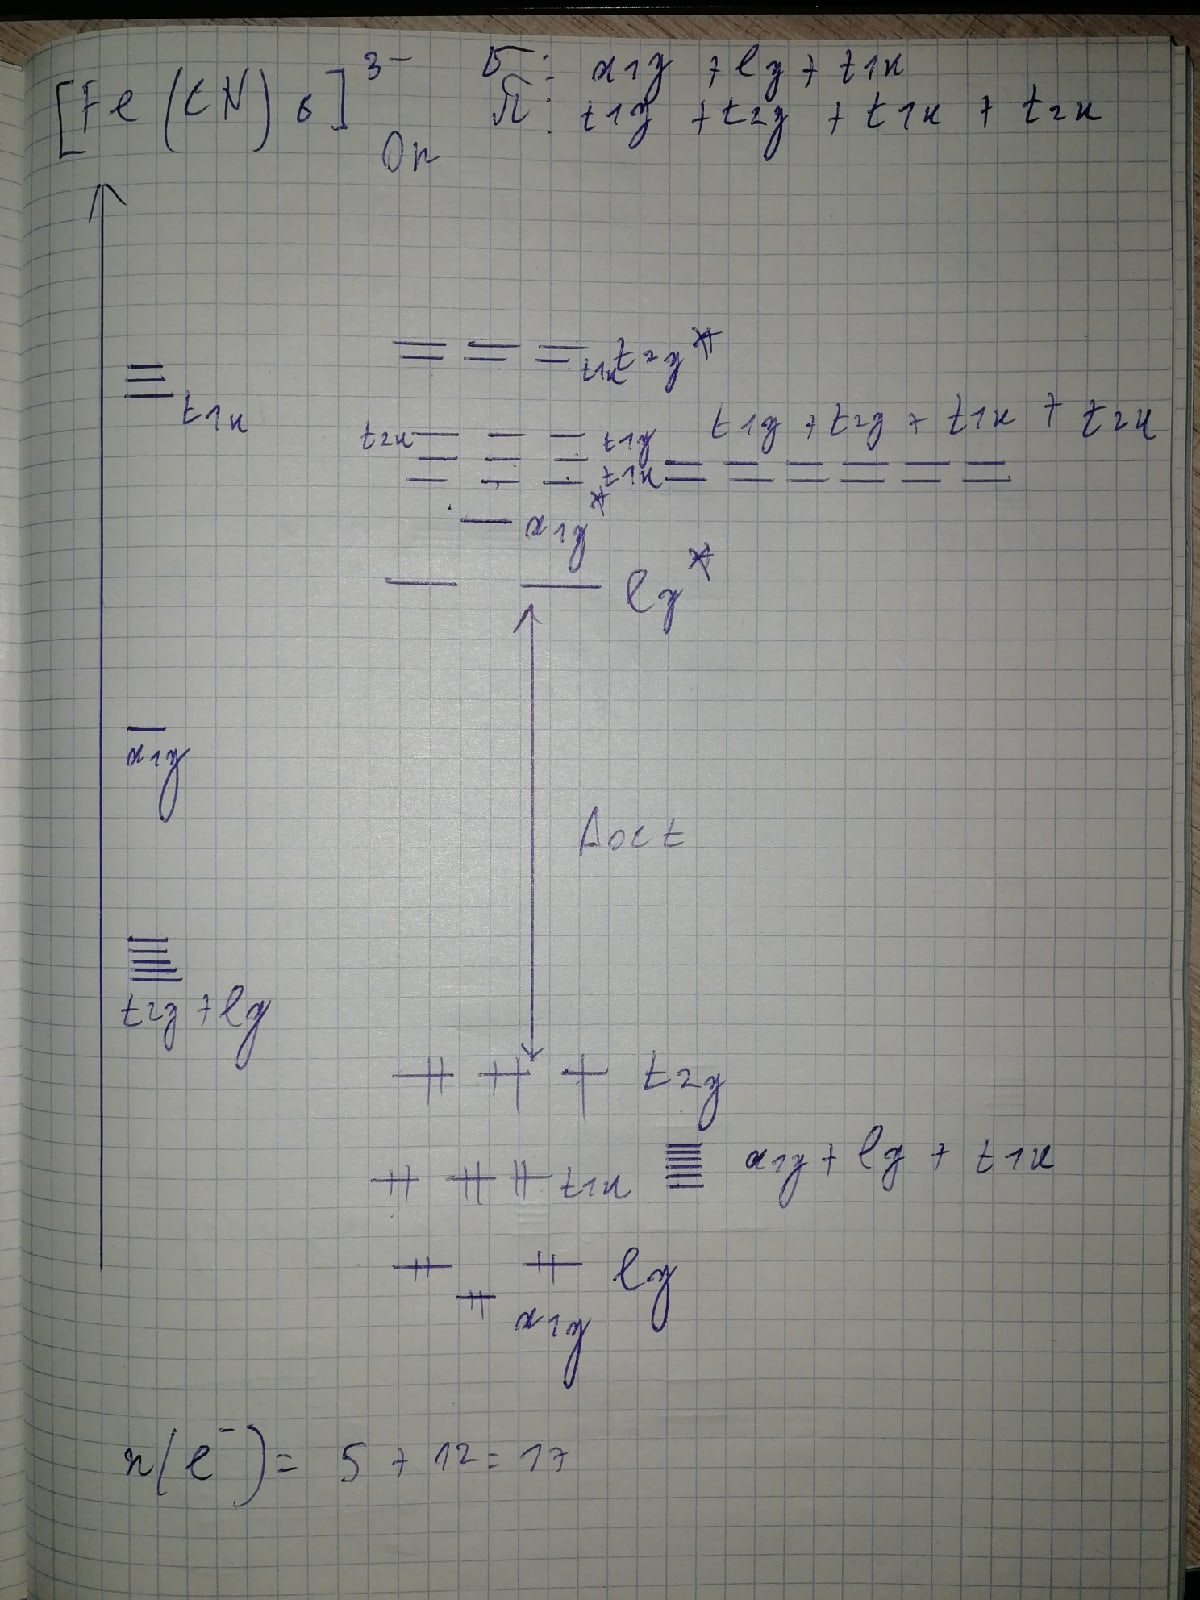
\includegraphics[scale=.300]{images/cyanides.jpg}
\end{figure}

Цианиды – лиганды сильного поля. Для 8 группы характерны октаэдрические комплексы, для 10 – квадратные. Начнём с 8 группы.

\subsubsection*{Красная кровяная соль(VIII гр.)}

Стоит отметить, что точную форму разрыхляющих орбиталей можно определить только с помощью оператора проектрирования, мы же основываем наши рассуждения на предположении, что разрыхляющие орбитали $CN^-$ взаимно-перпендикулярны, что не является грубым приблежением. Тогда симметрия аналогична галогенидным октаэдрическим комплексам. Разрыхляющие орбитали $CN^-$ расположены высоко по энергии, в силу чего поле в комплексе сильное.  ТКП с этим вполне согласна. ПС=5.5, Кс=0.9 


Отмечу, что при добавлении 1 электрона на связывающую орбиталь $t_{2g}$ мы получим анион жёлтой кровяной соли(ПС=1), что объясняет устойчивость $Fe^{2+}$ в комплексах с лигандами сильного поля. Окраска этих комплексов обусловлена другими факторами, так как перепрыгивание электрона на $e_g^*$-орбитали требует высокоэнергетической волны, длина которой, скорее будет в зоне ультрафиолета.

При переходе к рутению и осмию картина изменится несильно. Орбитали металла будут выше по энергии, перекрывание eg будет лучше, $t_{2g}$ – не сильно лучше, если не хуже. Это приведёт к увеличению энергетической щели.

\subsubsection*{Тетрацианидникель(X гр.)}
  
	Симметрия, опять-таки аналогична галогенидным квадратным коплексам. Интересно то, что с лигандами слабого поля $Ni^{2+}$ даёт тетраэдры, а с лигандами сильного поля – квадраты. Расщепление здесь соответсвтвует квадратному из ТКП. Отмечу, что орбиталь $b_{2g}$ будет  почти несвязывающей из-за плохого перекрывания. ПС=4, КС=1, комплекс диамагнитный. При переходе к палладию или платине картина почти не изменится, т.к. их орбитали выше, чем у никеля.
	
\begin{figure}[H]
\centering
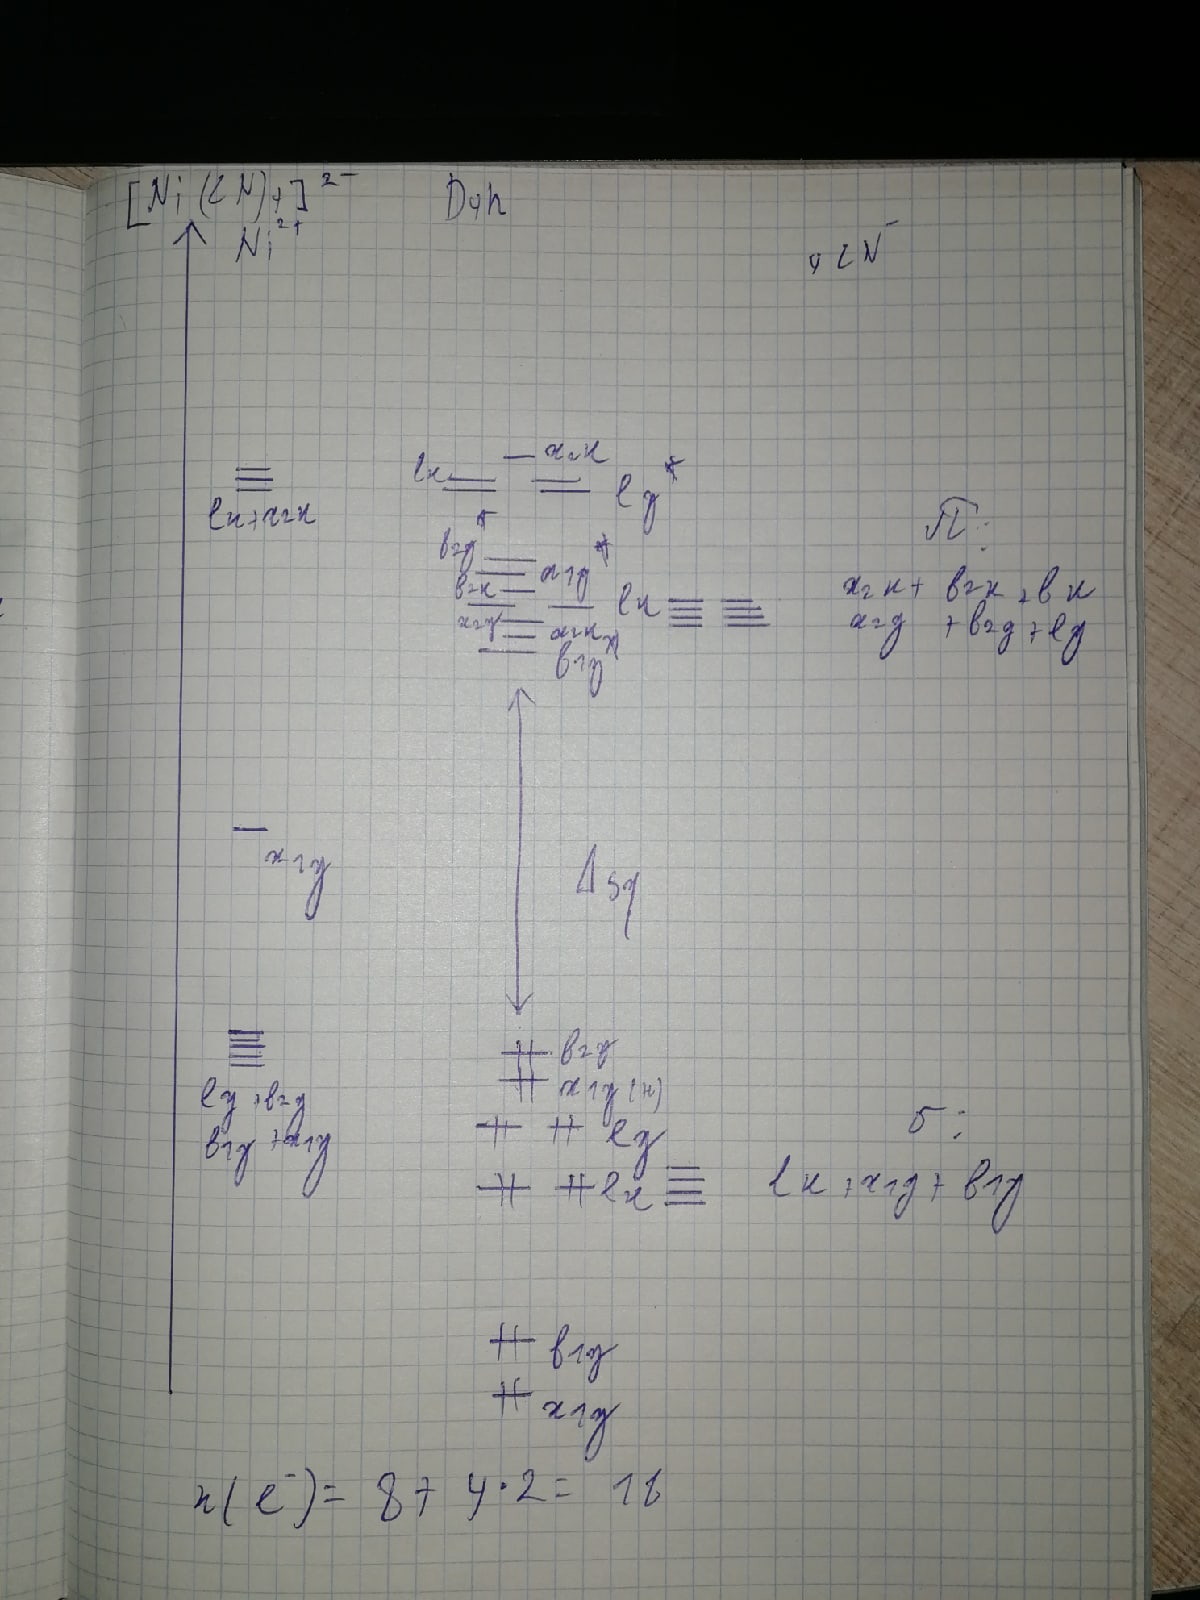
\includegraphics[scale=.300]{images/cyanides2.jpg}
\end{figure}
	